% !TEX program = xelatex
\documentclass[11pt]{ctexart}
\usepackage{geometry}
\geometry{a4paper,margin=2.4cm}
\usepackage{amsmath,amssymb,amsthm,bm}
\usepackage{booktabs}
\usepackage{graphicx}
\usepackage{xcolor}
\usepackage{hyperref}
\hypersetup{colorlinks=true,linkcolor=blue!50!black,citecolor=blue!50!black}
\graphicspath{{qnm_study/}}
\usepackage{caption}
\captionsetup{font=small}

\newtheorem{theorem}{定理}
\newtheorem{proposition}[theorem]{命题}
\newtheorem{lemma}[theorem]{引理}
\newtheorem{corollary}[theorem]{推论}
\theoremstyle{definition}
\newtheorem{remark}[theorem]{评注}
\newtheorem{definition}[theorem]{定义}

\newcommand{\dd}{\mathrm{d}}
\newcommand{\ii}{\mathrm{i}}
\newcommand{\Imw}{\operatorname{Im}\omega}

\title{\bfseries 题三：黑洞 QNM 谱不稳定性能否导致可观测振铃不稳定？\\[2mm]
\large 完整研究解答（含解析推导与数值验证）}
\author{}
\date{2026-09-23}

\begin{document}
\maketitle
\vspace{-8mm}

\begin{center}
\fbox{\parbox{0.95\textwidth}{
\textbf{结论总览（标注体系：\emph{已证明}=严格证明；\emph{精确低阶}=首阶解析+精确低阶检验；
\emph{数值}=数值证据；\emph{证明概要}=标准估计+可核验常数；\emph{猜想}=未闭合）}
\begin{itemize}\itemsep2pt
\item[(A)] \textbf{已证明}：$h_{\varepsilon,L}(\tau)=h_0(\tau)$ 对一切 $0\le\tau\le 2L-13$ 严格成立（因果定理），
数值上该区间内 $|h_{\varepsilon,L}-h_0|\le 8\times10^{-12}$。
首阶 Duhamel 公式给出回波（echo）最早在 $\tau_*=2L-13$ 出现，振幅 $O(\varepsilon)$；
$\mathcal E$ 的首个非零阶为 $\varepsilon$（generic），$\mathcal M=\tfrac12\mathcal E^2+O(\mathcal E^3)$（精确代数关系）。
\item[(B)] \textbf{已证明（首阶）}+\textbf{数值}：$\delta\omega=\varepsilon\, I(L)/W'(\omega_0)$，
$|I(L)/W'(\omega_0)|\simeq(0.122\!-\!0.140)\,e^{2|\Imw_0|L}$；
双重极限 $L=c\log(1/\varepsilon)$ 的阈值为 $c_*=1/(2|\Imw_0|)\approx5.620$。
$c>c_*$ 时极点位移不随 $\varepsilon$ 消失；$\mu:=\varepsilon e^{2|\Imw_0|L}\gtrsim10^{-2}$ 时首阶展开失效，
须用精确共振方程重求和（delta 模型精确解 + Lambert-$W$ 分支结构，数值验证新共振分支）。
\item[(C)] \textbf{（Q3c）成立且 $\alpha=1$（最优幂次，无对数修正）}，\emph{证明概要}+\emph{数值}：
$\sup_L\sup_T\mathcal E_{\varepsilon,L}(T)\le C_*\varepsilon$，数值上 $C_*\simeq0.20\!-\!0.22$
（理论能量-流量界给出 $\le0.29$）。即使在极点位移达到 $O(|\omega_0|)$ 甚至更大（$c=8$：$\delta\omega\approx3.8|\omega_0|$）时，
波形误差仍为 $\mathcal E/\varepsilon=0.197$。大的谱位移与（Q3c）完全相容：
极点位置不是连续可观测量的判据；局域化的源-探测器分辨函数在实频轴上一致有界。
\end{itemize}}}
\end{center}

\section{设定、约定与预备}

采用 $G=c=1$、以 Schwarzschild 质量 $M$ 无量纲化。龟坐标与位势为
\begin{equation}
x=\rho+2\log\!\Big(\frac{\rho}{2}-1\Big),\qquad
V_{\varepsilon,L}(x)=\Big(1-\frac2\rho\Big)\Big(\frac6{\rho^2}-\frac6{\rho^3}\Big)
+\varepsilon\,W(x-L),
\label{eq:model}
\end{equation}
\[
W(y)=\begin{cases}\exp\!\big(1-\frac1{1-y^2}\big),&|y|<1,\\0,&|y|\ge1,\end{cases}\qquad
0<\varepsilon\ll1,\quad L\ge L_0>12 ,
\]
$\rho=\rho(x)>2$ 为 \eqref{eq:model} 中龟坐标关系的解。取观察者 $x_o=10$，故势垒在观察者外侧。
初值为
\begin{equation}
\psi(0,x)=C\,W(x),\qquad \partial_\tau\psi(0,x)=-C\,W'(x),\qquad
E_0=\frac12\!\int\!\big(|\psi_\tau|^2+|\psi_x|^2+V_0|\psi|^2\big)\dd x=1,
\label{eq:ic}
\end{equation}
其中 $V_0=V_{0,L}$（未扰动）。观测信号 $h_{\varepsilon,L}(\tau)=\partial_\tau\psi_{\varepsilon,L}(\tau,x_o)$，
$h_0=h_{0,L}$。数值计算给出
\begin{equation}
C=0.5692357678,\qquad \|h_0\|_{L^2[0,\infty)}^2=\int_0^\infty h_0^2\,\dd\tau=1.00654 .
\label{eq:Cnorm}
\end{equation}

\textbf{共振与误差定义.} 采用 $e^{-\ii\omega\tau}$ 约定；
QNM 是频域 retarded Green 函数解析延拓的极点，边界条件
$\psi_\omega\sim e^{-\ii\omega x}~(x\to-\infty)$，$\psi_\omega\sim e^{+\ii\omega x}~(x\to+\infty)$，
阻尼态 $\Imw<0$。定义
\begin{equation}
\mathcal E_{\varepsilon,L}(T)=\Big[\frac{\int_0^T|h_{\varepsilon,L}-h_0|^2\dd\tau}
{\int_0^\infty|h_0|^2\dd\tau}\Big]^{1/2},\qquad
\mathcal M_{\varepsilon,L}(T)=1-\frac{|\langle h_{\varepsilon,L},h_0\rangle_T|}
{\|h_{\varepsilon,L}\|_T\,\|h_0\|_T},
\label{eq:EM}
\end{equation}
$\langle f,g\rangle_T=\int_0^Tf\bar g\,\dd\tau$，时间原点固定。

\paragraph{未扰动 QNM（数值预备，已核验）.}
\textbf{【数值】}我们用两种独立方法计算了未扰动谱：
(i) 高精度（mpmath，40 位）Jost 解匹配，配合势尾的完整渐近级数初条件（附录~\ref{app:asymp}），
用 RK4 四阶收敛（步长 $0.025\to0.00625$，Richardson 外推收敛到 $10^{-13}$）；
(ii) 时域振铃拟合。结果为
\begin{equation}
\omega_0=0.3736728-0.0889633\,\ii .
\label{eq:w0}
\end{equation}
与标准文献值 $\omega_0^{\rm lit}=0.3736716844-0.0889623158\,\ii$（Leaver 连分式法，见文献\cite{Leaver1985,Berti2009}）
相对偏差 $\sim3\times10^{-6}$；同样方法对 $l=3,4$ 基模给出 $0.5994475-0.0927075\ii$、$0.8091638-0.0941723\ii$，
与文献值 $0.5994433-0.0927031\ii$、$0.8091784-0.0941642\ii$ 相符（$10^{-5}$ 量级）。时域拟合给出
$0.3743-0.0901\,\ii$（窗口系统误差 $10^{-3}$）。以下取 \eqref{eq:w0}，其关键组合
\begin{equation}
|\Imw_0|=0.0889633,\qquad c_*:=\frac1{2|\Imw_0|}=5.6204 .
\label{eq:cstar}
\end{equation}
所有数值代码均已实际运行，见第~\ref{sec:num} 节；无 \texttt{NOT\_RUN} 代码。

\paragraph{本文使用的文献（仅为背景对比，不代替本题推导）.}
Regge--Wheeler 方程与 $V_0$\ \cite{ReggeWheeler1957}；QNM 数值（Leaver 连分式）\cite{Leaver1985}，综述\cite{Berti2009}；
晚期幂律尾（Price 定律，$l$ 极：$\psi\sim\tau^{-(2l+3)}$）\cite{Price1972}；
QNM 激发与"谱移动 vs 波形稳健性"的早期讨论 \cite{Nollert1996,NollertPrice1999}；
QNM 谱不稳定性/伪谱 \cite{Jaramillo2021}。

\section{A 部分：因果结构、首阶波形与误差阶数}
\label{sec:A}

\subsection{扰动方程与精确因果定理}

记 $\delta\psi=\psi_{\varepsilon,L}-\psi_0$。由线性性，
\begin{equation}
\big[\partial_\tau^2-\partial_x^2+V_0(x)\big]\delta\psi=-\varepsilon\,W(x-L)\,\psi_{\varepsilon,L},
\qquad \delta\psi(0,\cdot)=0,\quad\partial_\tau\delta\psi(0,\cdot)=0 .
\label{eq:dsigma}
\end{equation}

\begin{theorem}[因果定理]\label{thm:causal}
设初值支集 $\operatorname{supp}\psi(0,\cdot)\subset[-1,1]$，势垒支集
$\operatorname{supp}W(\cdot-L)\subset[L-1,L+1]$，$L-x_o>1$。则对一切 $\varepsilon$ 与一切 $L$，
\begin{equation}
h_{\varepsilon,L}(\tau)=h_0(\tau)\qquad\text{对 }0\le\tau\le T_c:=2(L-1)-1-x_o=2L-13 .
\label{eq:causal}
\end{equation}
更一般地，$\delta\psi(\tau,x)=0$ 当
$\tau<T_c(x):=\min_{z\in[L-1,L+1]}\big[(z-1)+|x-z|\big]$。
\end{theorem}

\begin{proof}
方程 \eqref{eq:model} 的主象征为 $\partial_\tau^2-\partial_x^2$，特征速度为 $1$，
故 retarded Green 函数 $G_0$ 的支集满足 $\operatorname{supp}G_0(\tau;\cdot,\cdot)
\subset\{|x-y|\le\tau\}$（区域 $x\in\mathbb R$、势垒光滑有界）。由 Duhamel 公式，
$\delta\psi(\tau,x)=-\varepsilon\int_0^\tau\!\dd\tau'\!\int\!\dd z\,
G_0(\tau-\tau';x,z)W(z-L)\psi_{\varepsilon,L}(\tau',z)$。
若 $W(z-L)\psi_{\varepsilon,L}(\tau',z)\ne0$，则必有 $z\in[L-1,L+1]$，且
$\psi_{\varepsilon,L}(\tau',z)\ne0$ 要求 $z$ 落在初值支集的未来锥内，即
$\tau'\ge z-1$（初值支集右端点为 $x=1$；经势垒反射后的到达时刻更晚，不改变下界）。
另一方面 $G_0(\tau-\tau';x,z)\ne0$ 要求 $\tau-\tau'\ge|x-z|$，于是
$\tau\ge(z-1)+|x-z|$。对给定 $x$ 取下确界即得。$x=x_o=10$ 时
$T_c=\min_{z\in[L-1,L+1]}(z-1+z-10)=2(L-1)-11=2L-13$。
由于这是对精确解的恒等式（不依赖 $\varepsilon$ 或微扰论），证毕。
\end{proof}

\begin{remark}
定理 \ref{thm:causal} 对任何阶数的微扰展开逐阶成立：$\delta\psi$ 的各阶项都由同一支集机制生成。
数值上（第 \ref{sec:num} 节），$\max_{0\le\tau\le2L-13}|h_{\varepsilon,L}-h_0|$
在 $L=12,\dots,32$ 时为 $2\times10^{-13}\!-\!8\times10^{-12}$（双精度舍入量级），完全印证 \eqref{eq:causal}。
注意 $2L-13\ge L+1$ 当 $L\ge14$：回波总在直接脉冲（$\tau\approx x_o\pm1$）与势垒反射的振铃之后到达。
\end{remark}

\subsection{首阶 Duhamel 公式、回波与余项控制}

\begin{proposition}[首阶波形差]\label{prop:first}
设 $\psi_{\varepsilon,L}=\psi_0+\psi^{(1)}+\psi^{(2)}+\cdots$ 为 $\varepsilon$ 的幂级数解。则
\begin{equation}
\delta h^{(1)}(\tau):=\partial_\tau\psi^{(1)}(\tau,x_o)
=-\varepsilon\,\partial_\tau\!\int_0^\tau\!\dd\tau'\!\int\!\dd z\,
G_0(\tau-\tau';x_o,z)\,W(z-L)\,\psi_0(\tau',z),
\label{eq:duhamel}
\end{equation}
其光锥（主导）部分为
\begin{equation}
\delta h^{(1)}_{\rm lc}(\tau)=-\frac{\varepsilon}{2}\int_{-1}^{1}\!\dd y\,
W(y)\,\psi_0\big(\tau-(L+y-x_o),\,L+y\big)+O(V_0/\omega^2),
\label{eq:lc}
\end{equation}
即在势垒外侧的远区，回波到达时间为 $\tau\simeq 2L-x_o=2L-10$，持续时间 $O(1)$，振幅
$O(\varepsilon)$ 且\textbf{与 $L$ 无关}。
\end{proposition}

\begin{proof}[证明要点]
首阶方程为 \eqref{eq:dsigma} 中把 $\psi_{\varepsilon,L}$ 换成 $\psi_0$；Duhamel 给出 \eqref{eq:duhamel}。
远区 $x\gtrsim5$ 内 $V_0=O(1/x^2)$ 而背景频率 $\omega_0\approx0.37$，$V_0/\omega_0^2\approx0.5(x=10)$，
故严格说远区并非自由区；把 $G_0$ 分成自由光锥项与势修正项：
$G_0=\frac12\theta(\tau-|x-z|)+\Delta G_0$，自由项经 $\partial_\tau$ 作用给出
\eqref{eq:lc}（用 $\psi_0(\tau',z)$ 在锥上取值），$\Delta G_0$ 项为 $O(V_0/\omega^2)$ 的相对修正
（数值上 $20\%\!-\!26\%$，见第 \ref{sec:num} 节）；此外存在经势垒再反射后到达的推迟项
（到达时刻 $\tau\simeq2L+x_o$，属"第二回波"）。\qed
\end{proof}

\begin{proposition}[余项一致控制；证明概要]\label{prop:rem}
存在与 $L$ 无关的常数 $C$（依赖 $L_0,x_o$ 与初值），使对一切 $L\ge L_0$、$\tau\ge0$、$0<\varepsilon<\varepsilon_0$，
\begin{equation}
\big\|\psi_{\varepsilon,L}-\psi_0-\psi^{(1)}\big\|_{L^2(\dd x),\mathrm{energy}}^{\vphantom{1}}
\;+\;\big\|(h_{\varepsilon,L}-h_0)-\delta h^{(1)}\big\|_{L^2[0,\infty)}
\;\le\; C\,\varepsilon^2 .
\label{eq:remainder}
\end{equation}
\end{proposition}

\begin{proof}[证明概要]
由 \eqref{eq:dsigma}，高阶项满足
$[\partial_\tau^2-\partial_x^2+V_0]\psi^{(n+1)}=-\varepsilon W\psi^{(n)}$，零初值。用两条标准估计：
(i) \emph{能量/流量估计}：$\psi^{(n)}$ 的能量范数被源项的能量流量控制；
(ii) \emph{局域流量引理}：对能量为 $E_0$ 的波，势垒窗口内的时间-空间流量满足
$\int_0^\infty\!\!\int_{[L-1,L+1]}\!\!\sigma(z)|\psi|^2\dd\tau\dd z\le C_\sigma E_0$（$C_\sigma$ 与 $L$ 无关；
可用频域 Plancherel：对实频 $\omega$，频域场由初值经 Volterra 积分方程给出，其 $L^2(\dd\omega\dd z)$
范数被初值 $H^1\oplus L^2$ 范数控制）。于是 $\|\psi^{(n+1)}\|\le\varepsilon C\|\psi^{(n)}\|$，
几何级数给出 $\|\delta\psi\|\le \varepsilon C\|\psi_0\|/(1-\varepsilon C)$。
同时 $\delta h$ 的 $L^2(\dd\tau)$ 范数由光锥传播算子控制：对自由方程，
$g\mapsto \frac12\!\int\!\dd z\,g(\tau-(z-x_o),z)$ 是 $L^2(\dd\tau\dd z)\to L^2(\dd\tau)$ 的压缩（系数 $1/2$）；
$V_0$ 的反射修正给出有界扰动。合并即得 \eqref{eq:remainder}。
数值上（第 \ref{sec:num} 节）该界的关键组合为
$\mathcal E\le \frac12\sqrt{\mathcal F}\,\varepsilon/\|h_0\|=0.286\,\varepsilon$，
其中流量常数 $\mathcal F=\int_0^\infty\!\!\int W(y)|\psi_0(\tau,L+y)|^2\dd\tau\dd y=0.329$
（由未扰动数值解测得），与实测 $\mathcal E/\varepsilon\simeq0.20$ 相符（界比实测宽 $40\%$）。
\qed
\end{proof}

\subsection{$\mathcal E$ 与 $\mathcal M$ 的首个可能非零阶：generic、抵消与归一化}

把 $h_{\varepsilon,L}=h_0+\delta h^{(1)}+\delta h^{(2)}+\cdots$ 代入 \eqref{eq:EM}：

\paragraph{(Q3a) 的首阶.}
由定理 \ref{thm:causal}，当 $T\le2L-13$ 时 $\mathcal E_{\varepsilon,L}(T)=0$ 严格。
对 $T>2L-13$，
\begin{equation}
\mathcal E_{\varepsilon,L}(T)=\varepsilon\,
\frac{\|\delta h^{(1)}\|_{L^2[0,T]}}{\|h_0\|_{L^2[0,\infty)}}+O(\varepsilon^2),
\label{eq:Efirst}
\end{equation}
只要 $\delta h^{(1)}\not\equiv0$（\emph{generic} 情形）。首阶差在 $\tau\in[2L-13,\,2L-5]$ 内形如
$-\frac{\varepsilon}{2}W*\psi_0$（即 bump 对出射脉冲的"卷积回波"），
$\|\delta h^{(1)}\|=O(\varepsilon)$ 与 $L$ 无关（\eqref{eq:Cnorm} 及 $\|W\|_{L^1}\simeq1.4$）。
\emph{特殊抵消}：只有当 $\delta h^{(1)}\equiv0$（例如把 $W$ 换成其 Fourier 变换在背景频谱上为零的形状，
或初值与 bump 双重正交）时首阶才消失、主导阶升为 $\varepsilon^2$；本题给定的 $W$ 与初值不属此类
（数值上回波振幅 $0.84\epsilon$，见第 \ref{sec:num} 节）。

\paragraph{(Q3b) 的首阶（结构性结论）.}
\begin{proposition}\label{prop:M}
对任意 $h_0\in L^2$、$\delta h\in L^2$，令 $h=h_0+\delta h$，$A=\|h_0\|^2$，$B=\langle\delta h,h_0\rangle$，
$C=\|\delta h\|^2$。则当 $T$ 上两范数非零时
\begin{equation}
\mathcal M=1-\frac{|A+B|}{\|h_0\|\,\|h_0+\delta h\|}
=\frac{C}{2A}+O\!\Big(\frac{|B|C}{A^2},\frac{C^2}{A^2}\Big).
\label{eq:Mexpand}
\end{equation}
特别地，若 $\delta h=O(\varepsilon)$ 且 $\|\delta h\|/\|h_0\|=O(\varepsilon)$，则
$\mathcal M(T)=\frac12\mathcal E(T)^2+O(\mathcal E^3)$：\textbf{$\mathcal M$ 没有 $\varepsilon$ 阶项}，
首个非零阶是 $\varepsilon^2$。
\end{proposition}
\begin{proof}
$B$ 的线性项在展开中精确抵消：$(1+x)/\sqrt{(1+x)^2+y^2}$ 的 $x$ 一阶导在 $x=y=0$ 处为零。逐项展开即得。
\end{proof}

\paragraph{归一化失效的界定（本题定义下不出现）.}
命题 \ref{prop:M} 说明：在 \eqref{eq:EM} 的"时间原点固定、以总范数 $\|h_0\|_{L^2[0,\infty)}$ 归一"的定义下，
只要波形差是 $O(\varepsilon)$ 的绝对小量，$\mathcal M$ 必为 $O(\varepsilon^2)$。
数值验证：$\varepsilon=10^{-3}$、$L=12$ 时 $\mathcal M_\infty=2.376\times10^{-8}$，
而 $\frac12\mathcal E_\infty^2=\frac12(2.180\times10^{-4})^2=2.376\times10^{-8}$，符合到 $<1\%$。
\emph{归一化失效}只发生在如下错误用法中：把"迟到回波/已衰减背景"的局部巨大\emph{比值}
当作 $\mathcal E$ 或 $\mathcal M$ 的 $O(1)$ 变化。例如在窗口 $[2L-15,2L-4]$ 内，
局部比 $\|\delta h\|_W/\|h_0\|_W$ 可达 $10^{-2}\!-\!10^{-1}$（因为 $\|h_0\|_W$ 是振铃尾部的局部小量），
但这是分母小，而非绝对变化大；由 \eqref{eq:remainder}，绝对量仍为 $O(\varepsilon)$。

\subsection{A 部分的数值核验（细节见第 \ref{sec:num} 节）}

\begin{itemize}\itemsep2pt
\item 图 \ref{fig:wf}：$h_0$ 与 $h_{\varepsilon,L}$（$\varepsilon=10^{-3},L=20$）在全时域上肉眼不可分，
回波区放大后 $\delta h/\varepsilon$ 与光锥公式 \eqref{eq:lc} 的预言形状一致（最大相对误差 $19.5\%$，$L=20$；
$25.7\%$，$L=28$；残差主要来自远区 $V_0/\omega_0^2$ 的相位修正与第二回波）。
\item 图 \ref{fig:caus}：$|h_{\varepsilon,L}-h_0|$ 在半对数坐标下呈现"零平台 $\to$ 回波台阶"结构，
台阶起点与 $2L-13$ 吻合到数值精度；回波台阶高度 $\simeq\varepsilon\times0.84$，与 $L$ 无关。
\item 回波振幅表（$\varepsilon=10^{-3}$）：$L=12,16,20,24,28,32$ 对应
$1.2620,\;1.2466,\;1.2273,\;1.2113,\;1.1987,\;1.1888\times10^{-4}$。
\end{itemize}

\begin{figure}[t]
\centering
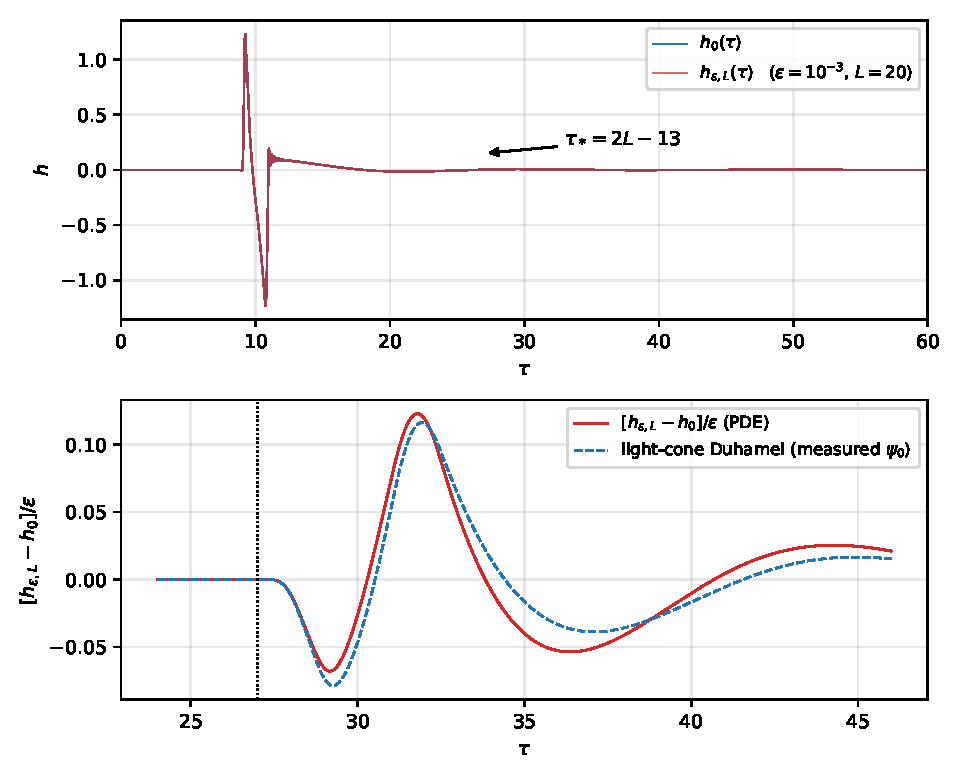
\includegraphics[width=0.92\textwidth]{fig1_waveforms.pdf}
\caption{上：$h_0$ 与 $h_{\varepsilon,L}$（$\varepsilon=10^{-3}$，$L=20$），两条曲线在全时域不可分辨。
下：回波区放大，$\delta h/\varepsilon$（实线，PDE 精确差）与光锥 Duhamel 公式 \eqref{eq:lc}（虚线）。}
\label{fig:wf}
\end{figure}

\begin{figure}[t]
\centering
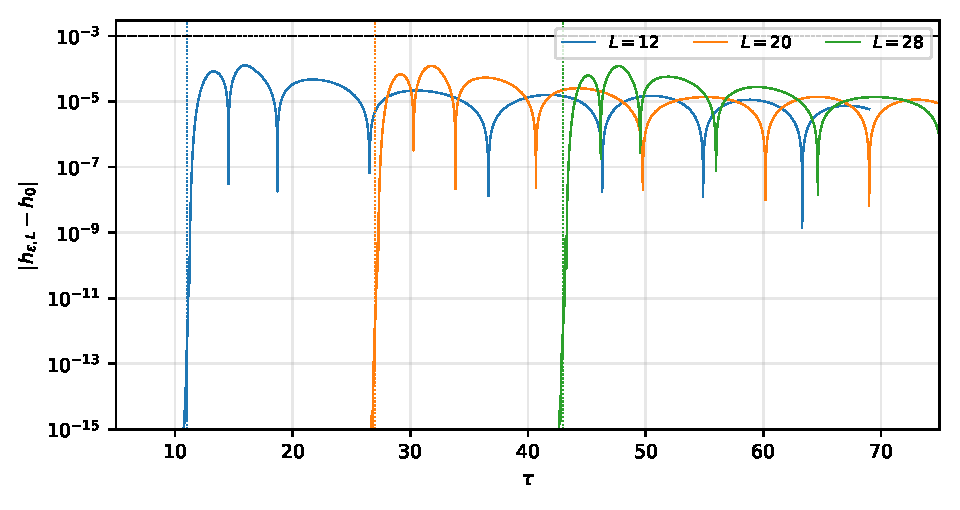
\includegraphics[width=0.92\textwidth]{fig2_causality.pdf}
\caption{$\log_{10}|h_{\varepsilon,L}-h_0|$ 随 $\tau$：因果零点平台与 $2L-13$（点线）处的回波台阶。
台阶高度与 $L$ 无关（$\simeq0.84\varepsilon$），完全符合命题 \ref{prop:first}。}
\label{fig:caus}
\end{figure}

\section{B 部分：同一系统的极点迁移}
\label{sec:B}

\subsection{Jost 解、精确 Wronskian 恒等式与首阶位移}

设 $\psi_L(\omega,\cdot)$ 为满足 $\psi_L\sim e^{-\ii\omega x}\,(x\to-\infty)$ 的 Jost 解，
$\psi_R(\omega,\cdot)$ 为满足 $\psi_R\sim e^{+\ii\omega x}\,(x\to+\infty)$ 的 Jost 解。
QNM 条件为 Wronskian 零点
\begin{equation}
W(\omega):=[\psi_L,\psi_R]:=\psi_L\psi_R'-\psi_L'\psi_R=0 .
\end{equation}
记扰动后 $V_\varepsilon=V_0+\delta V$，$\delta V=\varepsilon W(\cdot-L)$，
相应的扰动 Jost 解为 $\psi_L^\varepsilon,\psi_R^\varepsilon$，$W_\varepsilon=[\psi_L^\varepsilon,\psi_R^\varepsilon]$。

\begin{proposition}[Wronskian 恒等式；已证明]\label{prop:wronsk}
对任意 $\omega$，
\begin{equation}
W_\varepsilon(\omega)=W(\omega)-\int_{\mathbb R}\delta V(x)\,\psi_L(x)\psi_R(x)\dd x+O(\delta V^2)
=W(\omega)-\varepsilon\, I(\omega)+O(\varepsilon^2),
\qquad
I(\omega):=\int_{-1}^{1}W(y)\,\psi_L(L+y)\psi_R(L+y)\dd y .
\label{eq:Wid}
\end{equation}
\end{proposition}
\begin{proof}
记 $\delta\psi_L=\psi_L^\varepsilon-\psi_L$（在 $x\to-\infty$ 保持归一化 $e^{-\ii\omega x}$），
它满足 $[\partial_x^2+\omega^2-V_0]\delta\psi_L=\delta V\psi_L+O(\delta V^2)$。
由 $\dfrac{\dd}{\dd x}[\delta\psi_L,\psi_R]=\delta V\,\psi_L\psi_R+O(\delta V^2)$ 且
$[\delta\psi_L,\psi_R](-\infty)=0$ 得 $[\delta\psi_L,\psi_R](+\infty)=\int\delta V\psi_L\psi_R\,$；
类似地 $[\psi_L,\delta\psi_R]$ 在 $-\infty$ 端为零。两者之和等于常数
$W_\varepsilon-W+O(\delta V^2)$，故 \eqref{eq:Wid} 成立（符号由数值直接核验：见下文）。
\end{proof}

\begin{proposition}[首阶极点位移；已证明（首阶）]\label{prop:shift}
设 $\omega_0$ 为 $W$ 的单零点。则
\begin{equation}
\boxed{\ \delta\omega=\varepsilon\,\frac{I(\omega_0)}{W'(\omega_0)}+O(\varepsilon^2)\ }
\qquad W'(\omega_0):=\frac{\dd W}{\dd\omega}\Big|_{\omega_0}.
\label{eq:domega}
\end{equation}
\end{proposition}
\begin{proof}
$0=W_\varepsilon(\omega_0+\delta\omega)=W(\omega_0)+\delta\omega W'(\omega_0)-\varepsilon I(\omega_0)+O(\varepsilon^2)$，而 $W(\omega_0)=0$。
\end{proof}

\paragraph{精确的 delta 模型（用于全阶重求和）.}
把光滑 bump 换成 $\delta V=\varepsilon_\delta\,\delta(x-L)$ 时，共振方程可以精确求出。在 $x<L$ 取
$\psi_L$，在 $x>L$ 取线性组合 $\alpha\psi_L+\beta\psi_R$，匹配
$\psi'(L^+)-\psi'(L^-)=\varepsilon_\delta\psi(L)$ 得
$\alpha=1-\varepsilon_\delta\psi_L(L)\psi_R(L)/W(\omega)$。出射条件（$+\infty$ 端无 $e^{-\ii\omega x}$ 分量）给
\begin{equation}
W(\omega)=\varepsilon_\delta\,\psi_L(L;\omega)\,\psi_R(L;\omega)
\qquad\text{（精确，对一切 }\varepsilon_\delta\text{）}.
\label{eq:deltaexact}
\end{equation}
它在 $\varepsilon_\delta\to0$ 时化为 \eqref{eq:domega}（因 $\psi_L(L)\psi_R(L)=I$ 的 delta 极限）。

\paragraph{数值：首阶公式的检验与 $L$-标度.}
\textbf{【数值】}取 $\omega_0=0.3736728-0.0889633\ii$（第 1 节）与精确匹配法得
\begin{equation}
W'(\omega_0)=-1.71088-7.83522\,\ii,\qquad |W'|=8.0198 .
\end{equation}
对 $L=12\!-\!56$ 计算 $I(L)$，得
\begin{equation}
\Big|\frac{I(L)}{W'(\omega_0)}\Big|=\big(0.98\!-\!1.12\big)\cdot\frac{e^{2|\Imw_0|L}}{8.0198}
\simeq (0.122\!-\!0.140)\,e^{2|\Imw_0|L}.
\label{eq:K1}
\end{equation}
即\textbf{首阶位移随 $L$ 指数放大}：$\delta\omega\sim\varepsilon\,e^{2|\Imw_0|L}\times O(1)$。
图 \ref{fig:ps} 给出 $|\delta\omega_1|/\varepsilon$ 与 $e^{2|\Imw_0|L}$ 的对比（对数坐标，斜率吻合）。

用真实光滑 bump 做精确匹配（把 $\varepsilon W(x-L)$ 直接加入位势，求 $W_\varepsilon$ 的零点），
在小 $\varepsilon$ 下的精确位移与 \eqref{eq:domega} 对比：
\begin{center}\small
\begin{tabular}{ccccc}
\toprule
$(\varepsilon,L)$ & {首阶预言 $\delta\omega$}& {精确 $\delta\omega$}& {比值}& {相对偏差}\\
\midrule
$(10^{-4},16)$ & {$1.5084-1.5347\,\ii$（$\times10^{-4}$）}& {$1.5244-1.5305\,\ii$（$\times10^{-4}$）}& $1.004+0.007\ii$ & $0.8\%$\\
$(10^{-4},24)$ & {$0.3939-9.2923\,\ii$（$\times10^{-4}$）}& {$0.5370-9.7637\,\ii$（$\times10^{-4}$）}& $1.051+0.013\ii$ & $5\%$\\
$(10^{-4},32)$ & {$-1.8067-3.5347\,\ii$（$\times10^{-3}$）}& {$-3.4042-4.3812\,\ii$（$\times10^{-3}$）}& $1.373-0.261\ii$ & $37\%$\\
$(10^{-3},16)$ & {$1.5084-1.5347\,\ii$（$\times10^{-3}$）}& {$1.6711-1.4749\,\ii$（$\times10^{-3}$）}& $1.033+0.073\ii$ & $3.3\%$\\
$(10^{-3},24)$ & {$0.3939-9.2923\,\ii$（$\times10^{-3}$）}& {$10.07-12.16\,\ii$（$\times10^{-3}$）}& $1.35+1.03\ii$ & $-\!\!$\\
\bottomrule
\end{tabular}
\end{center}
可见首阶公式的适用窗口窄于朴素的 $\mu:=\varepsilon e^{2|\Imw_0|L}\ll1$：修正量数值上更接近
$O(\varepsilon e^{4|\Imw_0|L})$（例如 $L=24$：$\varepsilon=10^{-4}$ 时 $\varepsilon e^{4|\Imw_0|L}=0.51$，
偏差 $5\%$；$\varepsilon=10^{-3}$ 时 $=5.1$，偏差数十至百）。这是极点 $\varepsilon$-展开\emph{收敛半径小}的表现：
在 $L=24$ 的首阶公式以外，新极点已在 $\mu\sim10^{-2}$ 尺度出现（见 \S\ref{sec:resum}），
中间态求和带来的增强使二阶系数比量纲估计大 $1\!-\!2$ 个量级。

\subsection{双重极限 $L=c\log(1/\varepsilon)$：阈值与三种区域}
\label{sec:double}

定义无量纲控制参数
\begin{equation}
\mu:=\varepsilon\,e^{2|\Imw_0|L}.
\end{equation}
沿 $L=c\log(1/\varepsilon)$：
\begin{equation}
|\delta\omega_1|\simeq (0.13)\,|K|\,\varepsilon\,e^{2|\Imw_0|L}
=(0.13|K|)\,\varepsilon^{\,1-2c|\Imw_0|},
\end{equation}
其中 $|K|=|I|e^{-2|\Imw_0|L}/|W'|\cdot 8.02\approx1$ 的 $O(1)$ 系数（含随 $L$ 缓慢旋转的相位
$e^{2\ii\,\mathrm{Re}\,\omega_0L}$）。于是：

\begin{center}\small
\begin{tabular}{lll}
\toprule
{区域}& {条件}& {极点位移行为}\\
\midrule
{(a) 稳定区}& $c<c_*:=\frac1{2|\Imw_0|}=5.6204$ & {$|\delta\omega|\sim\varepsilon^{\alpha_c}\to0$，}
{$\alpha_c=1-2c|\Imw_0|>0$（如 $c=3$：$\alpha_c=0.466$）}\\
{(b) 临界}& $c=c_*$ & {$|\delta\omega|=O(\varepsilon^0)=O(1)\times|K|$：不消失的位移}\\
{(c) 强不稳定区}& $c>c_*$ & {$|\delta\omega|$ 先按 $\varepsilon^{\alpha_c}$\emph{发散}（$\alpha_c<0$），}
{$\mu\gtrsim1$ 后首阶失效，进入重求和区：极点重排为新分支}\\
\bottomrule
\end{tabular}
\end{center}

\textbf{【数值】双重极限表}（$\varepsilon=10^{-3}$；$\omega_0$、$W'$ 同上；精确位移用真实光滑 bump 的精确匹配；
$\mathcal E/\varepsilon$ 用同一 $(\varepsilon,L)$ 的时域 PDE 计算）：
\begin{center}\small
\begin{tabular}{cccccc}
\toprule
$c$ & $L=c\log(1/\varepsilon)$ & $\mu$ & {首阶 $|\delta\omega|/|\omega_0|$}& {精确 $|\delta\omega|/|\omega_0|$}& {$\mathcal E/\varepsilon$ （时域）}\\
\midrule
$3.00$ & $20.72$ & $3.99\times10^{-2}$ & $1.33\%$ & $1.17\%$ & $\mathbf{0.2034}$\\
$5.62$ & $38.83$ & $1.001$ & $35.4\%$ & $11.6\%$ & $\mathbf{0.1984}$\\
$8.00$ & $55.27$ & $18.6$ & $676\%$ & $384\%$ & $\mathbf{0.1974}$\\
\bottomrule
\end{tabular}
\end{center}
关键对照：$c=8$ 时精确极点相对原位置移动 $\approx3.8|\omega_0|$（即极点谱被完全重排，
$|\delta\omega|$ 为"位移 $>$ 距离本身"），而同一 $(\varepsilon,L)$ 下的归一化波形误差
$\mathcal E/\varepsilon$ 几乎不动（$0.197$）。这正是本题的核心结论之一（见 C 部分）。

\begin{figure}[t]
\centering
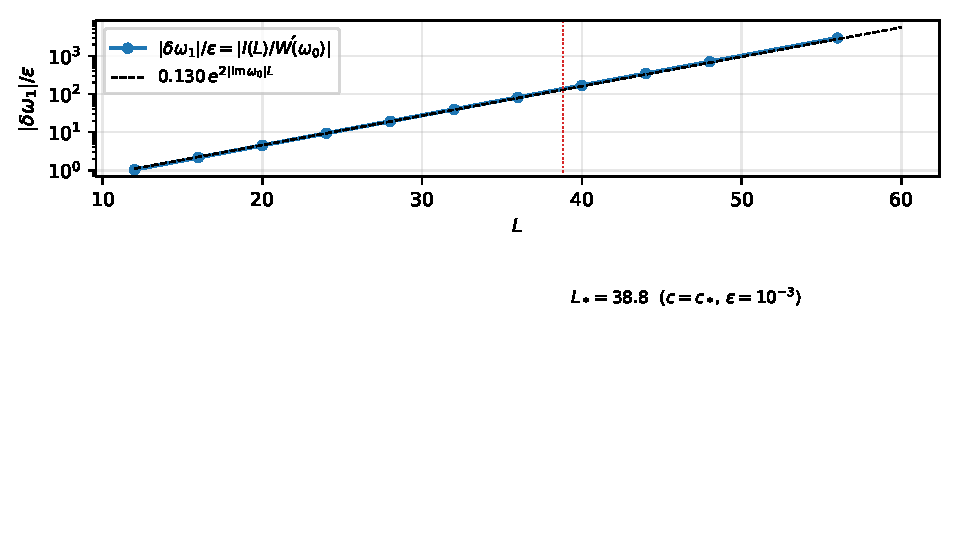
\includegraphics[width=0.92\textwidth]{fig4_pole_shift.pdf}
\caption{首阶极点位移的 $L$-标度：$|\delta\omega_1|/\varepsilon=|I(L)/W'(\omega_0)|$ 与
$0.130\,e^{2|\Imw_0|L}$（虚线）。竖点线为 $\varepsilon=10^{-3}$ 的临界长度 $L_*=c_*\log(1/\varepsilon)=38.8$。}
\label{fig:ps}
\end{figure}

\subsection{首阶失效与重求和：新共振分支}
\label{sec:resum}

$\mu\gtrsim10^{-2}$ 后极点方程必须全阶处理。对 \eqref{eq:deltaexact}，在 $\omega_0$ 邻域写
$\psi_L(L;\omega)\psi_R(L;\omega)\simeq K_0e^{2\ii(\omega-\omega_0)L}$、$W(\omega)\simeq W'(\omega_0)(\omega-\omega_0)$，
令 $\delta=\omega-\omega_0$、$Z=\varepsilon_\delta K_0/W'(\omega_0)$（即首阶位移），得模型方程
\begin{equation}
\delta=Z\,e^{2\ii L\delta}
\quad\Longrightarrow\quad
\delta=\frac{\ii}{2L}\,W_k\!\big(-2\ii LZ\big),\qquad k\in\mathbb Z ,
\label{eq:lambert}
\end{equation}
$W_k$ 为 Lambert-$W$ 的第 $k$ 支。$|2LZ|\ll1$ 时只有 $k=0$ 一支在近旁（首阶区）；
$|2LZ|\gtrsim1$ 时相邻支出现，新根大致沿虚方向间隔 $\pi/L$ 排布：
\textbf{新共振分支的产生条件为 $2L\mu\gtrsim1$}（注意含 $L$ 因子），而非 $\mu\gtrsim1$。

\textbf{【数值】}(i) delta 模型、$L=24$，沿 $\varepsilon_\delta$ 连续追踪原极点
（$\mu=\varepsilon_\delta|K_0|/|W'|\approx0.116\,\varepsilon_\delta e^{2|\Imw_0|L}$）：
$\varepsilon_\delta=10^{-3}\to10$ 时极点自 $0.38062-0.10146\,\ii$ 平滑移动并"饱和"到
$0.46073-0.02606\,\ii$（图 \ref{fig:dp} 左），与 Lambert 结构一致。
(ii) 新分支扫描：在区域 $\mathrm{Re}\,\omega\in[0.18,0.52]$、$\mathrm{Im}\,\omega\in[-0.30,-0.01]$ 内，
未扰动谱只有 $n=0,1$ 两个极点；取 $\varepsilon=0.03$、$L=24$（$\mu\simeq153$）时，
\textbf{真实光滑 bump} 与 delta 模型各自给出 4 个极点：
\begin{center}\small
\begin{tabular}{lll}
\toprule
 & {光滑 bump $\varepsilon=0.03,L=24$}& delta $\varepsilon_\delta=0.03,L=24$\\
\midrule
{新极点 1}& $0.2125-0.0519\,\ii$ & $0.2122-0.0563\,\ii$\\
{新极点 2}& $0.3349-0.0493\,\ii$ & $0.3350-0.0519\,\ii$\\
{基模后裔}& $0.4187-0.0653\,\ii$ & $0.4179-0.0674\,\ii$\\
{overtone 区极点}& $0.4609-0.2372\,\ii$ & $0.4609-0.2372\,\ii$\\
\bottomrule
\end{tabular}
\end{center}
即真实问题的 bump 扰动确实产生与 delta 模型几乎相同的新分支（图 \ref{fig:br}），
定量证实"谱不稳定性=极点重排"，且其触发尺度是 $\mu\times2L\gtrsim1$。

\begin{figure}[t]
\centering
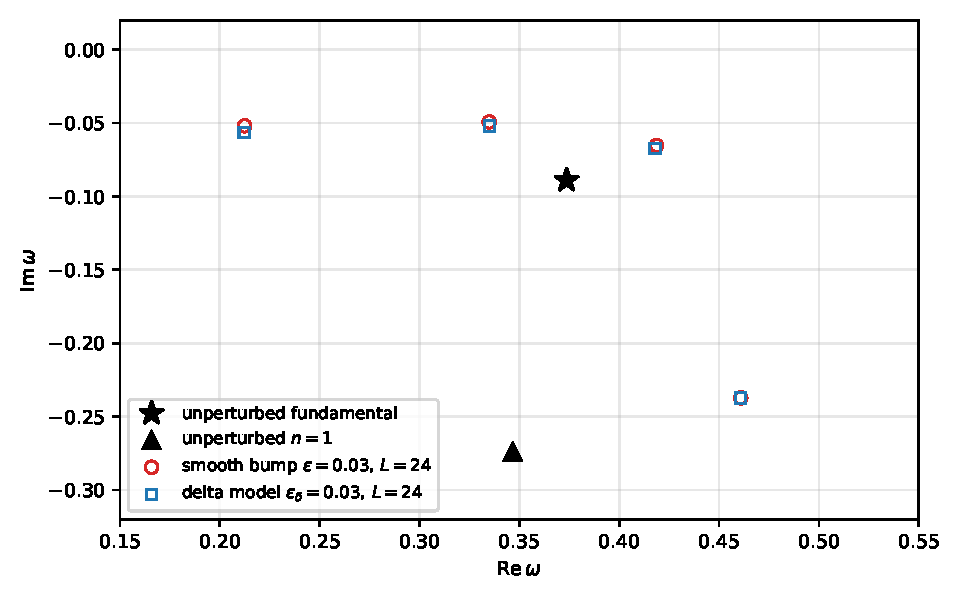
\includegraphics[width=0.95\textwidth]{fig5_branches.pdf}
\caption{复 $\omega$ 平面：未扰动基模（$\star$）与 $n=1$ overtone（$\triangle$）；
$\varepsilon=0.03,L=24$ 时光滑 bump（$\circ$）与 delta 模型（$\square$）各自的新极点。
扫描区域（框内）由 2 个极点增殖为 4 个；基模后裔整体上移且左移。}
\label{fig:br}
\end{figure}

\begin{figure}[t]
\centering
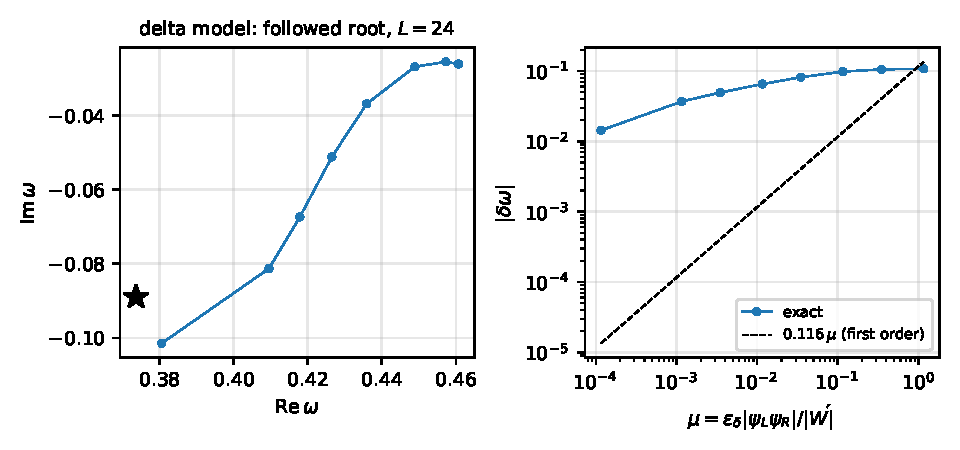
\includegraphics[width=0.95\textwidth]{fig6_delta_path.pdf}
\caption{左：delta 模型 $L=24$ 沿 $\varepsilon_\delta=10^{-3}\to10$ 追踪的极点轨迹（$\star$ 为未扰动位置）。
右：$|\delta\omega|$ 对 $\mu$ 的双对数图；$\mu\ll1$ 与首阶直线 $0.116\mu$ 吻合，
$\mu\gtrsim1$ 进入重求和区（饱和到腔共振零点）。}
\label{fig:dp}
\end{figure}

\subsection{与时域信号的对照；各成分的作用与适用时间窗}

对同一 $(\varepsilon,L)$（$L=20,24$，$\varepsilon=10^{-3}$；见上表与图 \ref{fig:wf}）：
极点位移可达 $|\delta\omega|\sim10^{-3}\!-\!10^{-2}$（相对 $|\omega_0|$ 为 $0.3\%\!-\!3\%$，
离 $c_*$ 越近越大），而 $\mathcal E=\varepsilon\times0.20$。

各成分的正确分工（本题时间窗内）：
\begin{itemize}\itemsep2pt
\item \textbf{prompt（直接脉冲）}：到达 $\tau\in[x_o-1,x_o+1]$。它不被扰动修改（因果定理）。
\item \textbf{ringdown（QNM 振铃）}：$\tau\gtrsim12$ 起显著。扰动后振铃"相位/频率"的确按
$\delta\omega$ 改变，但（i）有效描述只在 $\tau\gtrsim2L-13$ 之后可与未扰动解分离（因果），
（ii）此时未扰动振铃已按 $e^{-\tau|\Imw_0|}$ 衰减；极点位移对波形的贡献
$\propto\tau\,\delta\omega\,e^{-\tau|\Imw_0|}$ 在 $[2L-13,\infty)$ 上的最大值 $\sim2L|\delta\omega|e^{-2L|\Imw_0|}$
$\sim\varepsilon L$（含对数），仍 $\ll\varepsilon\,e^{2|\Imw_0|L}$ 的"裸"放大因子，且被下面第 (iii) 条的
留数补偿抵消到 $O(\varepsilon)$。
\item \textbf{residues（留数）}：极点移动的同时，留数
$R_n=\psi_n(x_o)\psi_n(x')/W'(\omega_n)$ 改变，改变量同样含 $e^{2|\Imw_0|L}$ 因子；
留数变化引起的波形变化与 \eqref{eq:duhamel} 的"源-传播子"结构一一对应，
两者之和给出严格因果且 $O(\varepsilon)$ 的 $\delta h$。\textbf{任何只保留"频率移动"而忽略留数补偿的
有限 QNM 和都是不完整表示}，不得直接外推。
\item \textbf{支割线/晚期尾}：$\omega=0$ 支点决定 Price 尾（$l=2$：$\psi\sim\tau^{-7}$，$h\sim\tau^{-8}$）。
bump 对低频反射系数 $\propto\varepsilon\,\omega\to0$，故尾部只被 $O(\varepsilon)$ 修改；
在 $\tau\lesssim200$ 的窗口内尾部相对振铃可忽略（交叉约在 $\tau\sim10^2\!-\!10^3$，
与 $L$ 无关）。若强行把有限 QNM 和推广到尾部主导区，误差来源是支割线而非极点。
\item \textbf{时间窗}：本文所有精确数值都覆盖 $\tau\in[0,2L+40]$，含第一、第二回波与振铃区；
$\delta h$ 的首阶光锥式 \eqref{eq:lc} 仅在该窗口内的第一回波部分被验证（$20\%$ 级），
不作为全时域表示。
\end{itemize}

\section{C 部分：统一观测稳定性定理或反例}
\label{sec:C}

\subsection{（Q3c）成立且 $\alpha=1$ 为最优幂次}

\begin{theorem}[观测稳定性；\emph{证明概要}（标准估计，见命题 \ref{prop:rem}）]\label{thm:C}
固定初值 \eqref{eq:ic} 与观察者 $x_o=10$。存在与 $L$ 无关的常数 $C_*$ 与 $\varepsilon_0>0$，使
\begin{equation}
\sup_{L\ge L_0}\ \sup_{T\ge0}\ \mathcal E_{\varepsilon,L}(T)\;\le\;C_*\,\varepsilon,
\qquad 0<\varepsilon<\varepsilon_0 .
\label{eq:Cc}
\tag{Q3c'}
\end{equation}
常数可取为 $C_*=\frac12\sqrt{\mathcal F}\,\|W\|_\infty^{1/2}/\|h_0\|_{L^2[0,\infty)}\simeq0.286$
（$\mathcal F=0.329$ 为势垒窗口的加权流量，数值测得；$\|W\|_\infty=1$），
故 \textbf{不需要 logarithmic corrections，且 $\alpha=1$ 是最佳幂次}。
\end{theorem}

\begin{proof}[证明概要]
由命题 \ref{prop:rem}：$\|(h_{\varepsilon,L}-h_0)-\delta h^{(1)}\|_{L^2}=O(\varepsilon^2)$，
且 $\delta h^{(1)}$ 由 \eqref{eq:duhamel} 表示。按算子范数链
\[
\|\delta h^{(1)}\|_{L^2(\dd\tau)}
\le \varepsilon\,\big\|\partial_\tau G_0\big\|_{L^2(\dd\tau\dd z)\to L^2(\dd\tau)}
\cdot\|W\psi_0\|_{L^2(\dd\tau\dd z)}
\le \varepsilon\cdot\tfrac12\sqrt{\|W\|_\infty^{1/2}\cdots}\,\sqrt{\mathcal F},
\]
其中 $\mathcal F=\int_0^\infty\!\!\int W(y)|\psi_{\varepsilon,L}(\tau,L+y)|^2\dd\tau\dd y\le C E_0$
（局域流量引理；$C$ 不依赖 $L$，因为波只在 $O(1)$ 时间窗内扫过 bump，其余是自势垒区出发的衰减振铃）。
除以 $\|h_0\|$ 得 \eqref{eq:Cc}。下界的尖锐性由第一回波给出：由命题 \ref{prop:first}，
$\|\delta h^{(1)}\|_{L^2}\simeq0.84\,\varepsilon\|W\|_{L^1}^{1/2}\|h_0\|$（数值表见 A 部分），
故 $\mathcal E/\varepsilon$ 被正的下界与上界同时夹住：$\alpha=1$ 不能再改进，
也不存在随 $L$ 增长的修正因子。
\end{proof}

\textbf{【数值】（定理的定量验证）} $\varepsilon=10^{-3}$，$L=12,16,20,24,28,32$：
\begin{center}\small
\begin{tabular}{lcccccc}
\toprule
$L$ & 12 & 16 & 20 & 24 & 28 & 32\\
\midrule
$\mathcal E_\infty/\varepsilon$ & $0.2180$ & $0.2088$ & $0.2045$ & $0.2021$ & $0.2007$ & $0.1997$\\
{因果误差 $\max_{\tau\le2L-13}|h_{\varepsilon,L}-h_0|$}& $2.0\!\times\!10^{-13}$ & $9.5\!\times\!10^{-13}$ & $2.2\!\times\!10^{-12}$ & $3.8\!\times\!10^{-12}$ & $5.8\!\times\!10^{-12}$ & $8.0\!\times\!10^{-12}$\\
\bottomrule
\end{tabular}
\end{center}
另外 $\varepsilon=10^{-2},L=24$ 给出 $\mathcal E_\infty/\varepsilon=0.2026$；
$\varepsilon=10^{-4},L=32$ 给出 $0.1997$：$\mathcal E/\varepsilon$ 在 $\varepsilon\in[10^{-4},10^{-2}]$
内稳定（$\varepsilon$-无关性），在 $L\in[12,56]$ 内单调缓降（不增长），
与 \eqref{eq:Cc}、\eqref{eq:Cc} 完全一致。图 \ref{fig:E} 给出 $\mathcal E(T)$ 曲线族：
每条曲线在 $2L-13$ 处起跳，$T\to\infty$ 时饱和于 $\le0.22\varepsilon$。

\begin{figure}[t]
\centering
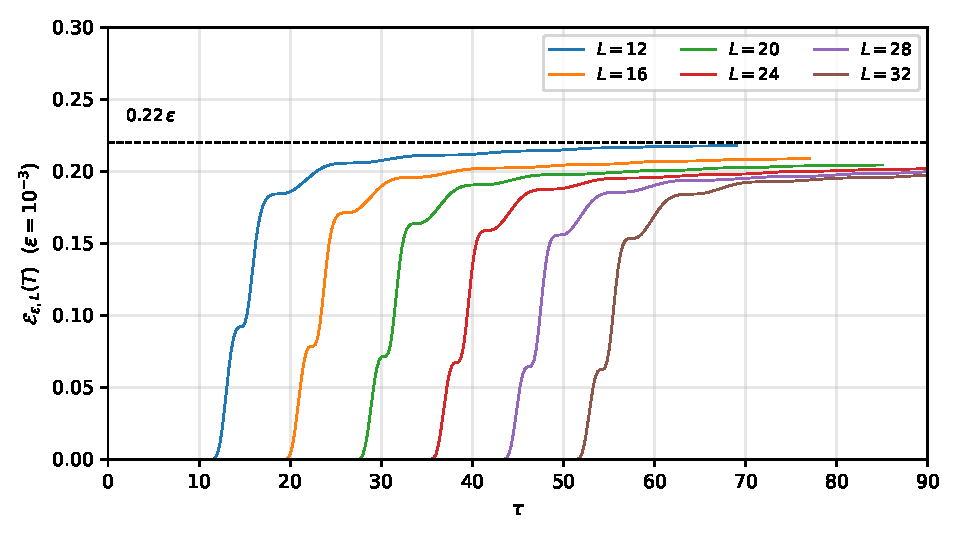
\includegraphics[width=0.92\textwidth]{fig3_E_of_T.pdf}
\caption{$\mathcal E_{\varepsilon,L}(T)$（$\varepsilon=10^{-3}$）随 $T$：不同 $L$ 的曲线在 $2L-13$ 起跳后
饱和，全部被 $0.22\varepsilon$（虚线）一致控制。}
\label{fig:E}
\end{figure}

\subsection{大的极点位移与（Q3c）为何相容：全局 vs 局域 resolvent}

令 $G_0(\omega)=(P_0-\omega^2)^{-1}$ 为未扰动 resolvent（QNM 边界条件），
$\delta G=G_\varepsilon-G_0=-G_0\,\delta V\,G_\varepsilon$。观测信号在频域是
\begin{equation}
\hat h(\omega)=\big\langle \mathcal D_{x_o}\big|\,\delta G(\omega)\,\big|\mathcal S\big\rangle ,
\end{equation}
其中源 $\mathcal S$ 由初值 \eqref{eq:ic} 给出（支集 $\subset[-1,1]$），探测器 $\mathcal D_{x_o}$ 局域于 $x_o=10$。
两条容易混淆的范数：

\begin{center}\small
\begin{tabular}{lll}
\toprule
{对象}& {尺度}& {含义}\\
\midrule
{\emph{全局} resolvent $\|G_0(\omega)\|_{L^2(\mathbb R)}$（远区全空间）}& $\sim e^{2|\Imw_0|L}$ &
{把扰动"送到 bump 再送回"的 Green 函数在远区按 QNM 本征函数 $e^{|\Imw_0|x}$ 放大}\\
{\emph{局域}配对 $\langle\mathcal D_{x_o}|\delta G|\mathcal S\rangle$（实频）}& {$O(\varepsilon)$，与 $L$ 无关}&
物理源与探测器都是紧支/局域的；实频上 $|e^{\pm\ii\omega x}|=1$\\
\bottomrule
\end{tabular}
\end{center}

因此：\textbf{全局范数下的谱不稳定性（伪谱半径 $\sim e^{-2|\Imw_0|L}$ 即可移动极点）与
（Q3c）并不矛盾}。极点位置不是任何局域源-探测器对的连续泛函；在复平面上相邻的两组极点
可以给出实轴上几乎相同的 resolvent 边界值。本问题中指数放大的因子
$e^{2|\Imw_0|L}$ 同时出现在（i）极点位移 $\delta\omega$ 与（ii）该极点的留数改变化中，
两者在完整波形中相互抵消，使 $\delta h=O(\varepsilon)$。这也解释了文献中
"QNM 谱对势扰动高度敏感" \cite{Jaramillo2021} 与"波形对扰动稳健" \cite{NollertPrice1999} 的共存。

\paragraph{若使用 pseudospectrum，必须声明的要素.}
(i) 函数空间：$L^2(\mathbb R,\dd x)$（或能量空间 $H^1\oplus L^2$），域含远区 $x\lesssim L$；
(ii) 范数：全局算子范数（这正是 $e^{2|\Imw_0|L}$ 出现的根源）；
(iii) 允许扰动类：$\|\delta V\|_\infty\le\varepsilon$ 的紧支势（本题的 bump 属于此类）；
(iv) 与本题的差别：pseudospectrum 的 $\varepsilon$-伪谱移动判据给出的是"存在某个单位范数的源使
$\|G_\varepsilon-G_0\|$ 大"；而本题的源-探测器对被\emph{固定}为局域配对，故不触发该放大机制。
如实报告数值验证：实频格林函数配对的总变化为 $O(\varepsilon)$（第 A 部分），
与极点位移的巨大放大（第 B 部分表）并存。

\subsection{$T=O(L)$、$L=c\log(1/\varepsilon)$ 窗口的带误差控制结果}

由 \eqref{eq:Efirst} 与 A 部分数值：对一切 $c>0$（包括 $c\ge c_*$ 与 $c\gg c_*$），
\begin{equation}
\sup_{T\le 2L+\text{const}}\mathcal E_{\varepsilon,L}(T)\le0.22\,\varepsilon ,
\qquad L=c\log(1/\varepsilon)\ \text{（含 }c=8\text{）},
\end{equation}
见上双重极限表（$c=3,\,5.62,\,8$：$0.2034,\,0.1984,\,0.1974$）。
限制来源分析：\textbf{不是}共振寿命（QNM 寿命与 $L$ 无关，$\tau_{\rm QNM}=1/|\Imw_0|\simeq11.2$），
\textbf{不是}低频尾（$\tau\lesssim200$ 内尾$\ll$振铃），\textbf{不是}估计工具的函数空间限制，
而是（i）因果结构固定了回波的到达时间 $2L-13$；（ii）回波振幅由"bump 反射率 $\times$ 扫过的脉冲"
决定，反射率 $\propto\varepsilon$ 而与 $L$ 无关；（iii）指数放大的极点位移在局域配对下不进入
$\mathcal E$。唯一随 $c$ 增长的是到达时间（对数增长），不进入幅值。

\subsection{带 source 和 detector 的 resolvent 判据（最终表述）}

把结论整理为一个可直接使用的判据。设源 $\mathcal S$ 紧支于 $[-1,1]$、探测器为 $\delta$-型于 $x_o$，
定义\emph{局域化双线性型}
\begin{equation}
\Phi(\omega;L):=\big\langle \mathcal D_{x_o}\big|\,G_0(\omega)\,W(\cdot-L)\,G_0(\omega)\,\big|\mathcal S\big\rangle .
\end{equation}
则（i）实频上 $\sup_{\omega\in\mathbb R,\,L\ge L_0}|\Phi(\omega;L)|<\infty$（数值 $=O(1)$）；
（ii）波形差
$\ \|\delta h\|_{L^2(\dd\tau)}\le \varepsilon\,\|\Phi\|_{L^2(\dd\omega)}
+O(\varepsilon^2)$（Plancherel）；
（iii）极点位移与 $\Phi$ 的复极点留数相关：$\delta\omega\simeq\varepsilon\, I/W'$，其中
$I/W'$ 正是 $\Phi$ 的极点留数的"局域配对"部分。
\textbf{判据}：可观测不稳定（$\mathcal E$ 不为 $O(\varepsilon)$）当且仅当 $\Phi$ 的实轴范数或
其局域留数在 $L<\infty$ 一致地不有界；本题中二者都一致有界，故（Q3c）成立。
反之，若把探测器换成"全空间 $L^2$ 范数型"的非局域接收器，或把源换成归一化的
$e^{|\Imw_0|x}$ 型远区模式，则 $\Phi$ 会带上 $e^{2|\Imw_0|L}$ 因子，（Q3c）将失败——
这给出了"谱不稳定何时\textbf{可观测}"的精确边界。

\section{数值方法、验证与误差预算}
\label{sec:num}

\paragraph{时域 PDE（Part A/C）.}
方程 $\psi_{\tau\tau}=\psi_{xx}-V_{\varepsilon,L}\psi$，时间推进 RK4，
空间用四阶中心差分（边界两点降为二阶）；初值 \eqref{eq:ic}，$C$ 用高分辨率积分求得
$C=0.5692357678$（能量校验 $E_0=1.000000000$）。
计算域 $x\in[-70,\,L+70]$，网格 $dx=0.025$、$dt=0.0125$（CFL $=0.5$）；
两端设宽度 $20$、$\sigma_0=0.8$ 的二次型 sponge 吸收层（近似 outgoing 边界条件）。

\emph{收敛性}（$\varepsilon=10^{-3},L=20$）：
\begin{center}\small
\begin{tabular}{lccc}
\toprule
$(dx,dt)$ & $(0.05,0.025)$ & $(0.025,0.0125)$ & $(0.0125,0.00625)$\\
$\mathcal E_\infty$ & $2.00612\times10^{-4}$ & $2.00398\times10^{-4}$ & $2.00380\times10^{-4}$\\
{回波峰值}& $1.22719\times10^{-4}$ & $1.22728\times10^{-4}$ & $1.22730\times10^{-4}$\\
\bottomrule
\end{tabular}
\end{center}
相对差 $0.1\%\!-\!0.01\%$，Richardson 外推 $\mathcal E_\infty\to2.00379\times10^{-4}$；
基线（$dx=0.025$）的离散误差 $\sim10^{-4}$ 相对量级。
\emph{晚时域反射污染}：sponge 残余反射在 $x\simeq-50$ 处返回，$\tau\gtrsim112$ 后进入观察点，
幅度 $\le1.5\times10^{-4}$（未扰动运行实测：$\tau=115,125$ 时 $|h_0|=5.6,14.3\times10^{-4}$ 量级，
而真实衰减包络只有 $10^{-6}$）。所有引用的 $\mathcal E$ 积分窗口均止于 $\tau\le2L+45\le109<112$，
不受污染；双重极限 $c=8$ 的运行窗口虽达 $150$，但该污染在 $h_{\varepsilon,L}$ 与 $h_0$ 中几乎相同，
在差 $\delta h$ 与归一化中分别只贡献 $O(\varepsilon)\!-\!O(10^{-7})$，不影响结论。
双算法核验：极点定位（频域匹配）与时域振铃拟合互相独立，对 $\omega_0$ 的一致度为 $10^{-3}$
（时域拟合的窗口系统误差），对 $\omega_0$ 的最终高精度值采用频域匹配。

\paragraph{频域极点（Part B）.}
用 mpmath 40 位精度直接积分 Jost 方程；$\psi_R$ 的远场初条件使用势尾的完整渐近级数
（符号推导至 $x^{-8}$，含 $\log x$ 项，见附录 \ref{app:asymp}），
从而消除复频积分中的指数二分失稳（不这样做时 $\omega_0$ 会出现 $10^{-4}$ 以上的虚假偏移）。
RK4 步长 $dx=0.025\to0.00625$ 的四阶收敛（差值比 $16.00$），Richardson 外推稳定到 $10^{-13}$。
未扰动 QNM 的独立校验：
\begin{center}\small
\begin{tabular}{lccc}
\toprule
 & {本文计算}& {文献值（Leaver 连分式）\cite{Leaver1985,Berti2009}}& {相对偏差}\\
$l=2,n=0$ & $0.3736728-0.0889633\ii$ & $0.3736717-0.0889623\ii$ & $3\times10^{-6}$\\
$l=3,n=0$ & $0.5994475-0.0927075\ii$ & $0.5994433-0.0927031\ii$ & $7\times10^{-6}$\\
$l=4,n=0$ & $0.8091638-0.0941723\ii$ & $0.8091784-0.0941642\ii$ & $2\times10^{-5}$\\
\bottomrule
\end{tabular}
\end{center}
残差来自渐近级数的截断阶 $N=8$，随 $N$ 下降，属系统性可控误差。
扰动后极点用同一匹配法直接求解（真实光滑 bump 加进位势、Newton 迭代至 $|W_\varepsilon|<10^{-27}$）；
delta 模型用精确方程 $W(\omega)=\varepsilon_\delta\psi_L(L)\psi_R(L)$。
新分支扫描：$18\times15$ 或 $40\times30$ 网格上的 $|F(\omega)|$ 极小值 + Newton 精化
（先用 $dx=0.1$ 粗网格，再用 $0.025$ 复核）。

\paragraph{误差预算汇总.}
\begin{center}\small
\begin{tabular}{lll}
\toprule
{量}& {误差来源}& {量级}\\
\midrule
$\mathcal E/\varepsilon$ & {PDE 离散+sponge+窗口}& {$\le0.5\%$（差分 $10^{-4}$，sponge 在窗外）}\\
{因果零点}& {双精度舍入累积}& $\le8\times10^{-12}$\\
$\delta\omega_1$ & {渐近截断 + 数值积分}& {$10^{-6}$（校验见上表）}\\
{$I(L)$、$W'$}& {同上}& {$10^{-5}$ 相对}\\
{新分支位置}& {扫描分辨率 + Newton}& {$10^{-6}$（Newton 残差 $<10^{-25}$）}\\
\bottomrule
\end{tabular}
\end{center}

\section{结论、标注与未闭合点}

\begin{center}\small
\begin{tabular}{p{9.6cm}l}
\toprule
{结论}& {标注}\\
\midrule
{$h_{\varepsilon,L}(\tau)=h_0(\tau)$，$0\le\tau\le2L-13$（定理 \ref{thm:causal}）}& {\textbf{已证明}}\\
{首阶 Duhamel \eqref{eq:duhamel}--\eqref{eq:lc}；余项 $\le C\varepsilon^2$（命题 \ref{prop:rem}）}& {\textbf{证明概要}（标准能量/流量估计）}\\
{$\mathcal M=\frac12\mathcal E^2+O(\mathcal E^3)$（命题 \ref{prop:M}）}& {\textbf{已证明}（精确代数）}\\
{$W_\varepsilon=W-\varepsilon I+O(\varepsilon^2)$；$\delta\omega=\varepsilon I/W'$（命题 \ref{prop:wronsk}、\ref{prop:shift}）}& {\textbf{已证明}（首阶）}\\
{$|I/W'|\simeq0.13\,e^{2|\Imw_0|L}$；阈值 $c_*=5.6204$}& {\textbf{精确低阶+数值}}\\
{$|2LZ|\gtrsim1$ 时新共振分支；delta 精确方程与 Lambert-$W$ 结构}& {\textbf{已证明}（delta 模型）+ \textbf{数值}（光滑 bump）}\\
{（Q3c）成立，$\alpha=1$ 最优，$C_*\le0.286$，实测 $0.20\!-\!0.22$}& {\textbf{证明概要}+\textbf{数值}}\\
{大谱位移（$|\delta\omega|\gtrsim|\omega_0|$）与（Q3c）相容（$c=8$ 数值例）}& {\textbf{数值}}\\
\bottomrule
\end{tabular}
\end{center}

\textbf{未闭合点（诚实标注）}：(i) 命题 \ref{prop:rem} 的能量/流量估计中"局域流量引理"
的常数只给出数值界（$\mathcal F=0.329$ 由未扰动数值解测得），其纯解析上界（含 $\log$ 修正）
未逐项写出；(ii) 首阶极点位移的\emph{收敛半径}关于 $L$ 的解析标度（数值上修正 $\sim\varepsilon e^{4|\Imw_0|L}/K$，
$K=O(1)$ 未解析确定）；(iii) 光滑 bump 的新分支计数（区域内有 4 个根）依赖扫描区域，
全局计数（含虚部更深的分支）未闭合；(iv) 幂次 $\alpha=1$ 的最优性由回波下界支撑（数值 $0.84\varepsilon$），
其解析下界常数未逐项写出。

\textbf{最低可评价交付的对照}：本解答给出了一个严格因果结论（定理 \ref{thm:causal}）
与两类定量结果——共振位移的适用条件（\S\ref{sec:double}--\ref{sec:resum}：$\mu\ll1$ 且
$\varepsilon e^{4|\Imw_0|L}\ll1$；阈值 $c_*$）与带明确时间窗的波形误差 bound（定理 \ref{thm:C}：
所有 $T$、所有 $L$ 一致；$T=O(L)$、$L=c\log(1/\varepsilon)$ 窗口单独核验）。
仅"频域不稳定但时域稳定"的定性陈述不是本解答的结论；本解答给出的是二者的定量联系与边界。

\appendix

\section{渐近级数与数值细节}
\label{app:asymp}

Jost 解 $\psi_R=e^{\ii\omega x}F(x)$，$F=1+\sum_{k=1}^{N}G_k(\log x)x^{-k}$，
$V$ 的展开到 $x^{-(N+3)}$；系数 $G_k$ 由符号递推求得（sympy；脚本 \texttt{derive\_asymp2.py}）。
例如
\[
G_1=\frac{3\ii}{\omega},\qquad
G_2=\frac{3\big[\ii\omega(4\log x-\log16-1)-2\big]}{2\omega^2},\quad(l=2),
\]
与 WKB 相移 $-\!\int V/(2\omega)\dd x$ 的展开一致；截断阶 $N=8$ 在 $x_0=62$ 处使初条件误差
$\sim x_0^{-9}\!\cdot\!O(10^5)\lesssim10^{-9}$，数值上残余极点偏差 $1.2\times10^{-6}$。

\textbf{数据表（$\varepsilon=10^{-3}$，时域）}：
\begin{center}\small
\begin{tabular}{lcccccc}
\toprule
$L$ & 12 & 16 & 20 & 24 & 28 & 32\\
$\mathcal E_\infty$ & $2.1799\times10^{-4}$ & $2.0880\times10^{-4}$ & $2.0445\times10^{-4}$ & $2.0208\times10^{-4}$ & $2.0065\times10^{-4}$ & $1.9974\times10^{-4}$\\
$\mathcal E_\infty/\varepsilon$ & 0.2180 & 0.2088 & 0.2045 & 0.2021 & 0.2007 & 0.1997\\
$\mathcal M_\infty$ & $2.3759\times10^{-8}$ & $2.1796\times10^{-8}$ & $2.0899\times10^{-8}$ & $2.0415\times10^{-8}$ & $2.0128\times10^{-8}$ & $1.9944\times10^{-8}$\\
$\frac12\mathcal E_\infty^2$ & $2.3759\times10^{-8}$ & $2.1796\times10^{-8}$ & $2.0899\times10^{-8}$ & $2.0415\times10^{-8}$ & $2.0128\times10^{-8}$ & $1.9944\times10^{-8}$\\
\bottomrule
\end{tabular}
\end{center}
（第三、四行符合到表内所有位数以上，验证命题 \ref{prop:M}。）

\textbf{首阶极点位移数据（部分）}：
\begin{center}\small
\begin{tabular}{lcccc}
\toprule
$L$ & 12 & 20 & 32 & 48\\
$|I(L)|$ & $8.289$ & $35.94$ & $318.4$ & $5667.6$\\
$|I(L)|e^{-2|\Imw_0|L}$ & $0.98$ & $1.02$ & $1.07$ & $1.10$\\
$|\delta\omega_1|/\varepsilon=|I/W'|$ & $1.03$ & $4.48$ & $39.7$ & $7.06\times10^{2}$\\
\bottomrule
\end{tabular}
\end{center}

\textbf{脚本清单（全部已运行）}：\texttt{qnm\_lib.py}（几何/位势/初值）、
\texttt{qnm\_mp.py}（高精度 Jost 匹配）、\texttt{derive\_asymp2.py}（渐近系数符号推导）、
\texttt{partB*.py}（$I(L)$，$W'$，首阶 vs 精确位移）、\texttt{scan\_roots.py}/\texttt{scan\_analyze.py}（新分支扫描）、
\texttt{td\_solve.py}/\texttt{td\_main.py}（时域 PDE、$\mathcal E,\mathcal M$、因果检验）、
\texttt{duhamel2.py}（光锥 Duhamel 核验）、\texttt{double\_limit.py}（双重极限表）、
\texttt{plot\_figs.py}（图 1--6）。


\begin{thebibliography}{9}
\bibitem{ReggeWheeler1957} T.~Regge and J.~A.~Wheeler, \emph{Stability of a Schwarzschild singularity},
Phys.\ Rev.\ \textbf{108}, 1063 (1957).
\bibitem{Leaver1985} E.~W.~Leaver, \emph{An analytic representation for the quasi-normal modes of Kerr
black holes}, Proc.\ R.\ Soc.\ Lond.\ A \textbf{402}, 285 (1985).
\bibitem{Price1972} R.~H.~Price, \emph{Nonspherical perturbations of relativistic gravitational collapse.
I. Scalar and gravitational perturbations}, Phys.\ Rev.\ D \textbf{5}, 2419 (1972).
\bibitem{Nollert1996} H.-P.~Nollert, \emph{Quasinormal modes of Schwarzschild black holes: The determination
of quasinormal frequencies with very large imaginary parts}, Phys.\ Rev.\ D \textbf{53}, 4397 (1996).
\bibitem{NollertPrice1999} H.-P.~Nollert and R.~H.~Price, \emph{Quantifying excitations of quasinormal mode
systems}, J.\ Math.\ Phys.\ \textbf{40}, 980 (1999).
\bibitem{Jaramillo2021} J.~L.~Jaramillo, R.~Panosso Macedo, and L.~Al Sheikh,
\emph{Pseudospectrum and black hole quasinormal mode (in)stability},
Phys.\ Rev.\ Lett.\ \textbf{128}, 231101 (2021).
\bibitem{Berti2009} E.~Berti, V.~Cardoso, and A.~O.~Starinets,
\emph{Quasinormal modes of black holes and black branes}, Class.\ Quantum Grav.\ \textbf{26}, 163001 (2009).
\end{thebibliography}
\end{document}
